\documentclass[11pt,a4paper,man,floatsintext]{apa6}

\usepackage[english]{babel}
\usepackage[utf8]{inputenc}
%\usepackage[colorinlistoftodos]{todonotes}
\usepackage{graphicx,bm,hyperref,amsmath,amssymb}
%\usepackage{natbib} % necessary for bibtex
\usepackage{float}
\usepackage{url}
\usepackage{subfigure}
\usepackage{multirow}
\usepackage{csquotes}
\usepackage[table,xcdraw]{xcolor}
\usepackage[
backend=biber,
style=apa,
citestyle=numeric
]{biblatex}

\addbibresource{myRefs.bib}

\linespread{1.5}
\title{\large{Emotion Detection from Text: Effects of the Number of Categories on Accuracy}}
\shorttitle{Emotion Detection From Text}
\author{Jacky Lin, Melissa Tjong, Chengcheng Ding, Hanzheng Wang}
\affiliation{Department of Computer Science, \\Bucknell University, \\
Lewisburg, PA 17837}
\date{\today}

\begin{document}
\maketitle

\section{Abstract}

In this paper, we focus on detecting multiple categories of feelings based on text. These feelings include but are not limited to anger, fear, happiness, sadness, and surprise. We design and implement the neural network that imitates the human ability of text-based empathy of emotions. We use existing data sets to train and test our neural network. Each data set we use contains information on texts and their corresponding emotions. The goal of this neural network is to predict human emotion based on the input sentence. We also compare the performance between different numbers of categories.

\newpage

\section{Introduction}
Emotion detection is a sub-field of sentiment analysis, which deals with identifying emotions from sources. People express emotions in various ways, including facial expressions, spoken expression, writing or typing expression, and physiological expression. Due to the prosperity of social networks, communications between people are increasingly relying on typing or texting. Such a phenomenon has made emotion detection from text one of the most intriguing areas within emotion recognition. Although this area is a relatively nascent research area, many works have been published with diverse types of neural networks. Tripto and Ali \cite{lstmeg} use a Long Short Term Memory networks (LSTM) architecture within their deep learning model to detect sentiment from Bangla sentence. Cai and Hao \cite{Cai} tried to detect emotions from Weibo, a popular Chinese microblogging site, by using the Bidirectional LSTM model, which allows the networks to have both backward and forward information about the sequence at every time step. Jayakrishnan et al. \cite{svmeg} classify sentences in Malayalam novel into five emotions with a support vector machine (SVM), a supervised machine learning model. Huang et al. \cite{breteg} include methods of both LSTM and Bidirectional Encoder Representations from Transformers (BERT) to detect emotions in tweets.

This paper is presenting one way of detecting emotions from text using a Bidirectional LSTM model. We train and test this model using two existing data sets, International Survey on Emotion Antecedents and Reactions (ISEAR) \cite{ISEAR}, and Tweets \cite{TweetData}. We also compare our model's performance with the different number of sentimental categories in scope of accuracy and loss.

\section{Implementation}

\subsection{Data Sets}
In this project, we use two data sets contains sentences labeled with sentiments to train our model and test accuracy after training. Two data sets are International Survey on Emotion Antecedents and Reactions (ISEAR) and Tweets. The differences and characteristics of the two data sets are:
\begin{enumerate}
    \item Besides sentences labeled with sentiments, ISEAR includes much detailed information related to personal information, such as country, city, sex, and so on, as well as information related to details of occurrence of emotions such as how long a certain emotion remains, the intensity of certain emotions. In contrast, Tweets is relatively simpler. Besides sentences labeled with sentiments, it contains users' information, including user id and user name. For simplicity, in this project, we only use sentences and their labeled sentiments without using any non-anonymous information in consideration for privacy protection.
    \item The perspective of expressions in both data sets differs. Sentences in ISEAR corresponding to different emotions are descriptions of events in third-person perspectives, while sentences in tweets are a direct expression of emotions in first-person perspectives. For example, "I want to be a hero" is a direct expression of enthusiasm, while "when I watch heroic films" is a description of an event when this person expresses his or her feelings.
    \item There are seven categories of emotions in the ISEAR data set with around 1000 data for each type. Tweets, in comparison, have 13 categories of emotions with a total number of data of 40000. However, the number of data for each type varies from 100 to 8000, which is unevenly distributed. (See Fig.~\ref{datadist})
\end{enumerate} 

\begin{figure}[H]
\hfill
\subfigure{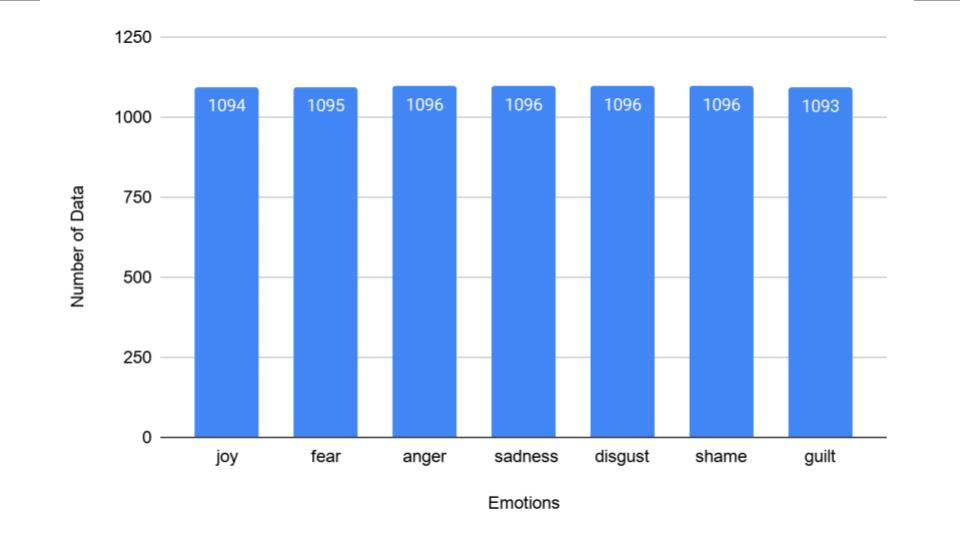
\includegraphics[width=3in]{img/ISEARDist.jpg}}
\hfill
\subfigure{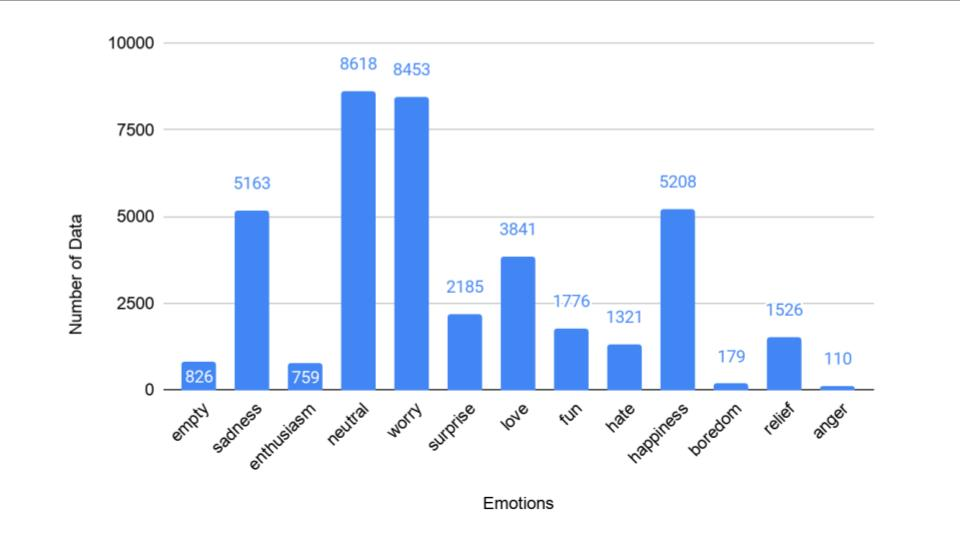
\includegraphics[width=3in]{img/TweetsDist.jpg}}
\hfill
\caption{Distribution of Two Data Sets\label{datadist}}
\end{figure}

\subsection{Models}
The neural network we use in this project is implemented using many types of layers. This section introduces some characteristics of these layers and how these features facilitate emotion detection from text.

The first model we use is GloVe Embedding Layer. GloVe \cite{GloVe} is a model for distributed word representation. The model is an unsupervised learning algorithm for obtaining vector representations for words. The GloVe model is trained on the non-zero entries of a global word-word co-occurrence matrix, which tabulates how frequently words co-occur with one another in a given corpus. An example is that ice co-occurs more frequently with solid than it does with gas. When we process natural language, consideration of co-occurrence of words helps machines conduct a human-like feature abstraction from the text.

The second model is Bidirectional LSTMs (Bi-LSTM), which is an extension of traditional LSTMs. This model is capable of learning long-term dependencies. Long-term dependencies refer to connecting previous information to the present task, which is suitable for context analysis in this project. Bi-LSTMs train two instead of one LSTMs on the input sequence. The first on the input sequence as-is and the second on a reversed copy of the input sequence. Bi-LSTMs can provide additional context to the network and result in faster, and even fuller learning on the problem \cite{bilstm}.

% Besides the implementation of layers, we also use some matrices and optimization to compile the model

% \begin{enumerate}
%     \item Optimizer: Adam Optimization: Adam is an optimization algorithm that can be used instead of the classical stochastic gradient descent procedure to update network weights iterative based in training data.
%     \item Text preprocessing: We implemented a series of methods including but not exclusively type error checking, removing stopwords, and lemmatization. (tutorial: \cite{NLP_tutorial})
%     \item Loss function: Categorical crossentropy: Crossentropy loss, measures the performance of a classification model whose output is a probability value between 0 and 1. This crossentropy loss function is used when there are two or more label classes. We expect labels to be provided in a one hot representation.
%     \item Matrix: categorical accuracy: categorical accuracy checks to see if the index of the maximal true value is equal to the index of the maximal predicted value.
% \end{enumerate}

%%%%%%%%%% add structure fig
The structure of our neural network is showing below (See Fig.~\ref{struct}). The input part is a GloVe embedding layer, which is set to be non-trainable, and a Gaussian noise layer which is to add some noises to the data in order to add some robustness to the neural network. Then the core of the neural network contains one Bidirectional LSTM, which strives to obtain features from the text in cooperation with the context of inputs, and two dropout layers as a method of regularization aiming to avoid over-fitting. Finally, our model's output is two dense layers with activation function of ReLu and Softmax, both of which serve to interpret the output from LSTM and make predictions.

\begin{figure}[H]
\centering

\includegraphics[width=6in]{img/NeuralNetworkStructure.jpg}
\caption{Structure of Neural Network
\label{struct}}
\end{figure}


\section{Result}

We train our neural network with different data sets with various categories. The performance is shown in Tab.~\ref{perform}. These results indicate that the more categories to classify, the lower the accuracy and the higher the loss. There is a negative correlation between the number of categories and the accuracy of training, validation, and testing. With thirteen categories, we have only $33.62\%$ accuracy. At the same time, the accuracy of the model improves to $61.46\%$ with seven categories. When classifying only three categories, the model has an accuracy of $95.35\%$. Generally speaking, when we half the number of categories each time, the accuracy of classification by this model increases by around $30\%$.

\begin{table}[ht]
 \caption{Best Performance on Each Training Sets\label{perform}}
\centering
\begin{tabular}{|c|c|c|c|c|c|c|}
\hline
dataset & cat. & max train acc. & max valid acc. & test acc. & min train loss & min valid loss \\ \hline
ISEAR & 7 & 0.5832 & 0.6146 & 0.615 & 1.1491 & 1.1812 \\ \hline
\multirow{2}{*}{Tweets} & 13 & 0.351 & 0.3362 & 0.336 & 1.8851 & 1.9411 \\ \cline{2-7} 
 & 3 & 0.837 & 0.9535 & 0.95 & 0.4226 & 0.0998 \\ \hline
\end{tabular}
\end{table}



\section{Ethical concerns}

There are several reasons that we believe that our result may be in one or more ways 'biased':
\begin{enumerate}
    \item Linguistic analysis takes the environment into account, and depending on the environment, these analyses may be affected by cultural stereotypes.
    \item How are we able to use data that is representative of a larger population? ISEAR database contains responses from people in multiple countries, but both those responses and tweets are in English.
    \item This leads to data that is skewed towards a more Western perspective, which could possibly lead to a negative emotional association of these texts with minority groups.
    \item It is difficult to accurately classify specific emotions, especially with data that is highly variable, such as tweets
\end{enumerate}
However, at this stage, it is almost impossible to incorporate data from non-western countries since they speak different languages. Hence, this is practically an inevitable bias that we will have to admit in our project. Therefore, We must stress that this model is not guaranteed to be precise for different cultural groups. We would advise that such models are used only for suggestive purposes instead of the sole source of judgment.

\section{Conclusion}

There are several challenges in this paper. First, when we have a relatively larger number of emotions, this model shows an unsatisfying accuracy, where the accuracy stops growing at an early stage of training. Another challenge is that other factors don’t affect much of the prediction in the ISEAR data set. Therefore, future works can focus on developing more complex or deeper neural networks to detect more specific emotion types or use multiple input neural networks to account for other factors involving the data set. From an ethical perspective, although this model is already satisfactory in predicting emotion in text into three categories as positive, negative, and neutral, we admit that the resulting model can be biased against certain groups and advise that such models are used only for suggestive purposes instead of the sole source of judgment. 

\printbibliography
\end{document}
